\documentclass[compress]{beamer}
\usepackage{ifthen,verbatim}

\newcommand{\isnote}{}
\xdefinecolor{lightyellow}{rgb}{1.,1.,0.25}
\xdefinecolor{darkblue}{rgb}{0.1,0.1,0.7}

%% Uncomment this to get annotations
%% \def\notes{\addtocounter{page}{-1}
%%            \renewcommand{\isnote}{*}
%% 	   \beamertemplateshadingbackground{lightyellow}{white}
%%            \begin{frame}
%%            \frametitle{Notes for the previous page (page \insertpagenumber)}
%%            \itemize}
%% \def\endnotes{\enditemize
%% 	      \end{frame}
%%               \beamertemplateshadingbackground{white}{white}
%%               \renewcommand{\isnote}{}}

%% Uncomment this to not get annotations
\def\notes{\comment}
\def\endnotes{\endcomment}

\setbeamertemplate{navigation symbols}{}
\setbeamertemplate{headline}{\mbox{ } \hfill
\begin{minipage}{5.5 cm}
\vspace{-0.75 cm} \small
\end{minipage} \hfill
\begin{minipage}{4.5 cm}
\vspace{-0.75 cm} \small
\begin{flushright}
\ifthenelse{\equal{\insertpagenumber}{1}}{}{Jim Pivarski \hspace{0.2 cm} \insertpagenumber\isnote/\pageref{numpages}}
\end{flushright}
\end{minipage}\mbox{\hspace{0.2 cm}}\includegraphics[height=1 cm]{../cmslogo} \hspace{0.1 cm} \includegraphics[height=1 cm]{../tamulogo} \hspace{0.01 cm} \vspace{-1.05 cm}}

\begin{document}
\begin{frame}
\vfill
\begin{center}
\textcolor{darkblue}{\Large Proposed Constants for Muon Alignment}

\vfill
\begin{columns}
\column{0.3\linewidth}
\begin{center}
\large
\textcolor{darkblue}{Jim Pivarski}

\vspace{0.2 cm}
Alexei Safonov
\end{center}
\end{columns}

\begin{columns}
\column{0.3\linewidth}
\begin{center}
\scriptsize
{\it Texas A\&M University}
\end{center}
\end{columns}

\vfill
27 January, 2009

\end{center}
\end{frame}

%% \begin{notes}
%% \item This is the annotated version of my talk.
%% \item If you want the version that I am presenting, download the one
%% labeled ``slides'' on Indico (or just ignore these yellow pages).
%% \item The annotated version is provided for extra detail and a written
%% record of comments that I intend to make orally.
%% \item Yellow notes refer to the content on the {\it previous} page.
%% \item All other slides are identical for the two versions.
%% \end{notes}

\small

\begin{frame}
\frametitle{Recommended constants}
\begin{itemize}\setlength{\itemsep}{0.25 cm}
\item Minor modification of the CRAFT\_ALL\_V4 (first re-processing):
  correct the $r\phi$ positions of the highest-statistics chambers
\begin{itemize}
\item pattern of residuals versus $\phi$, $z$ indicates a chamber-by-chamber phenomenon
\item alignment study used tracks from the TIB and TOB only (most trusted)
\item rigorous fitting procedure insensitive to $\vec{B}$-field errors
  and variation of track distribution across chamber surface
\item passes a track-based validation with unbiased residuals (following slides)
\item tested by Javier (this is the .db on CASTOR)
\end{itemize}

\end{itemize}
%% \hspace{-0.83 cm} \textcolor{darkblue}{\Large Outline2}
\end{frame}

\begin{frame}
\frametitle{Example residuals plot}

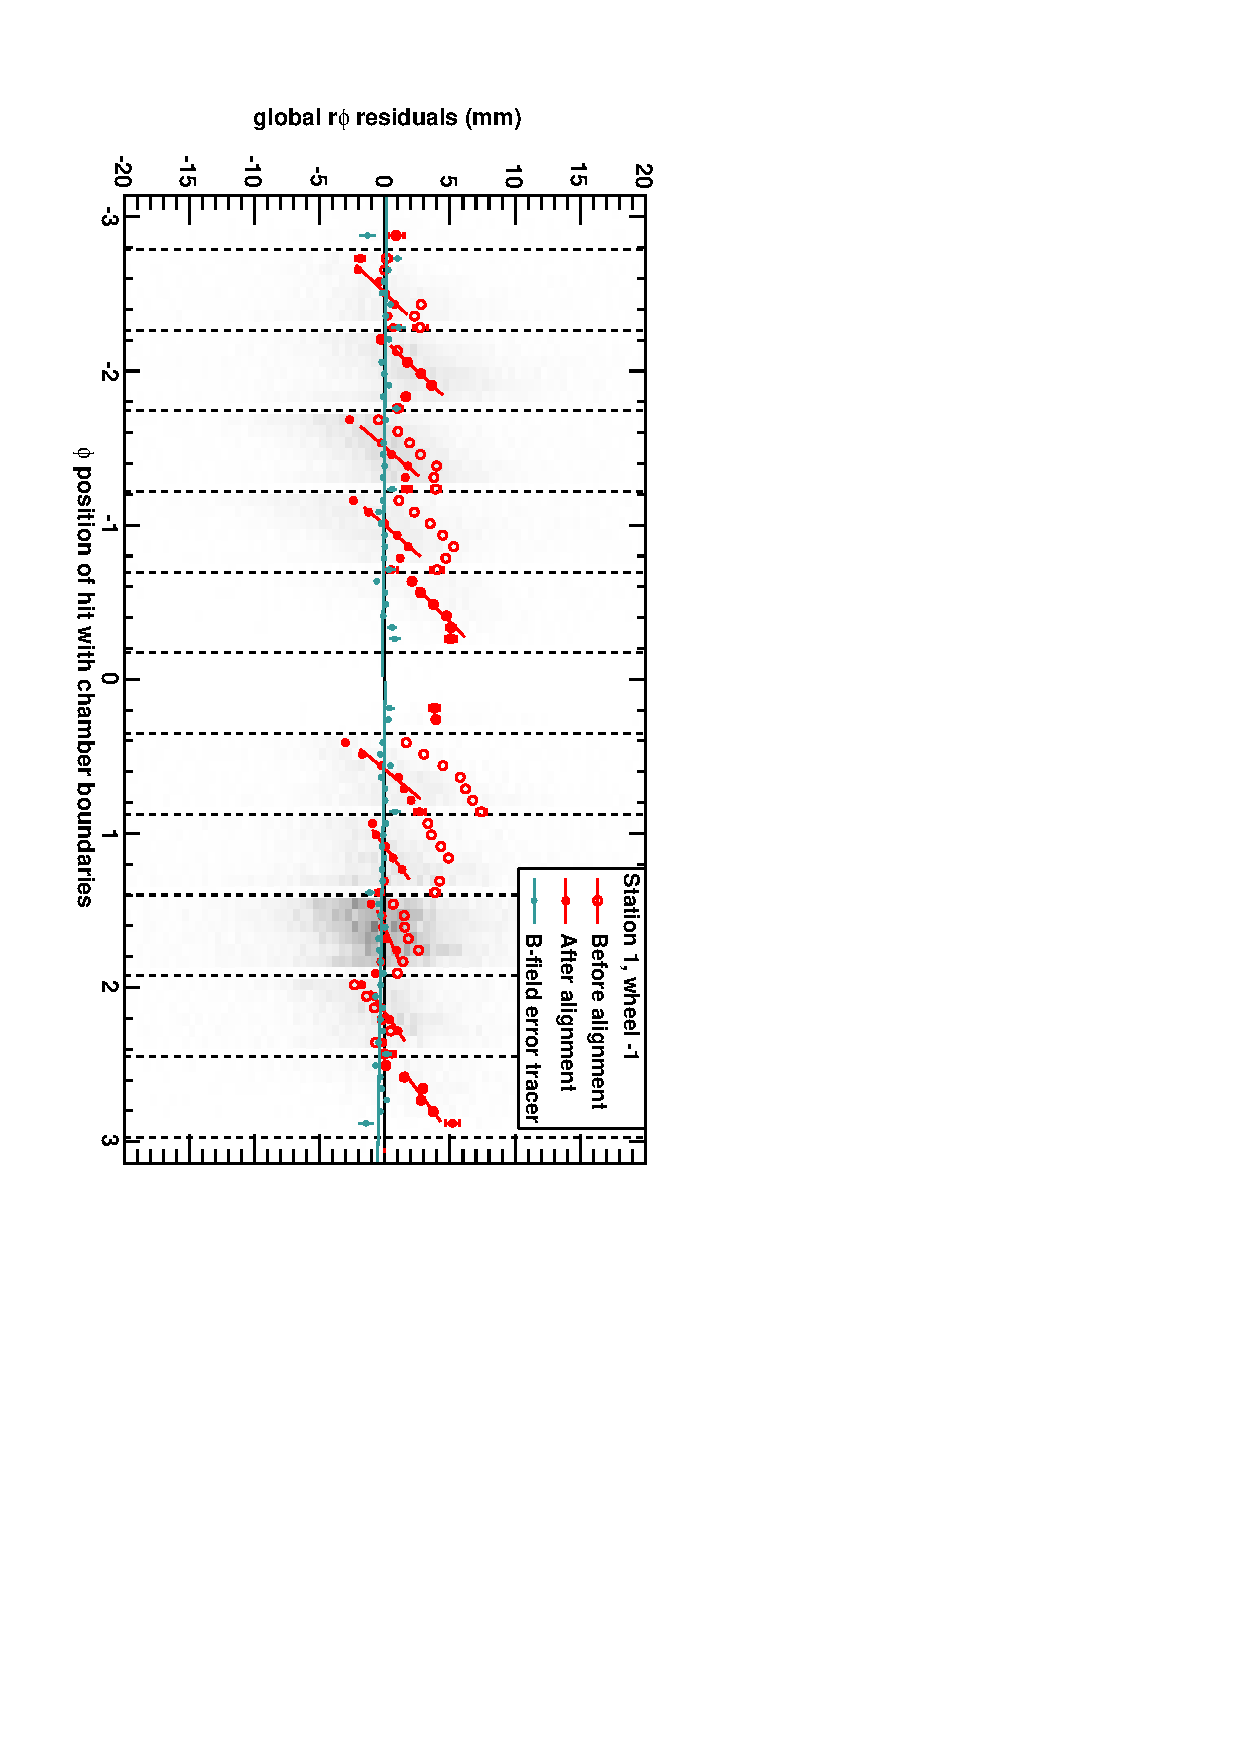
\includegraphics[height=\linewidth, angle=90]{DTrphiVsPhi_st1_whB.pdf}

\begin{itemize}
\item Alignment moved center of chambers to zero in $r\phi$ (note:
  center of {\it chambers,} not center of mass of track distribution)
\item ``Sawtooth mountain'' shape is still there, because we didn't do
  anything to correct for it
\end{itemize}
\end{frame}

\begin{frame}
\frametitle{Other projection}

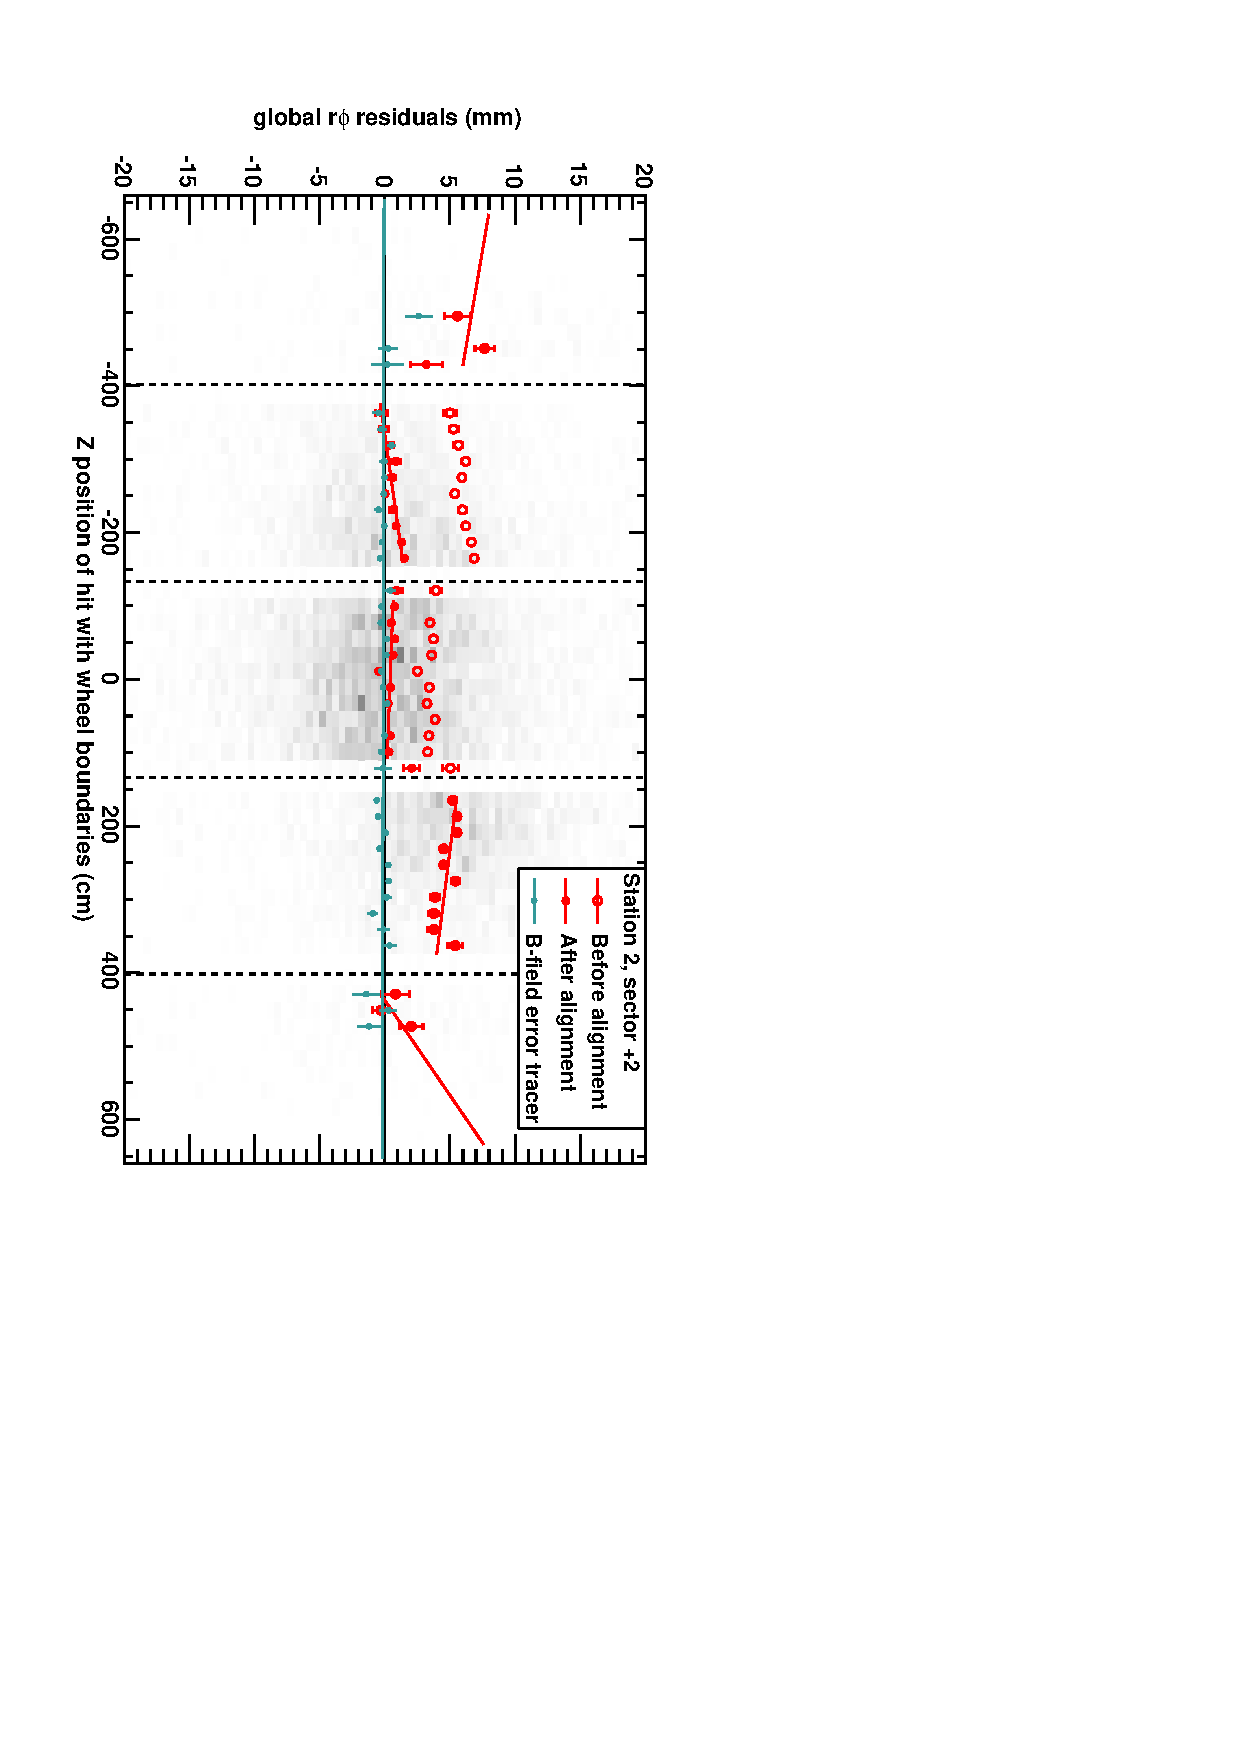
\includegraphics[height=\linewidth, angle=90]{DTrphiVsZ_st2_sr02.pdf}

\begin{itemize}
\item Makes sense in the vs.\ $z$ projection as well
\item Not all chambers were aligned, only the ones with at least 800
  well-distributed tracks (overly conservative?)
\end{itemize}
\end{frame}

\begin{frame}
\frametitle{Residuals summary}

\begin{columns}
\column{0.3\linewidth}
Station 1

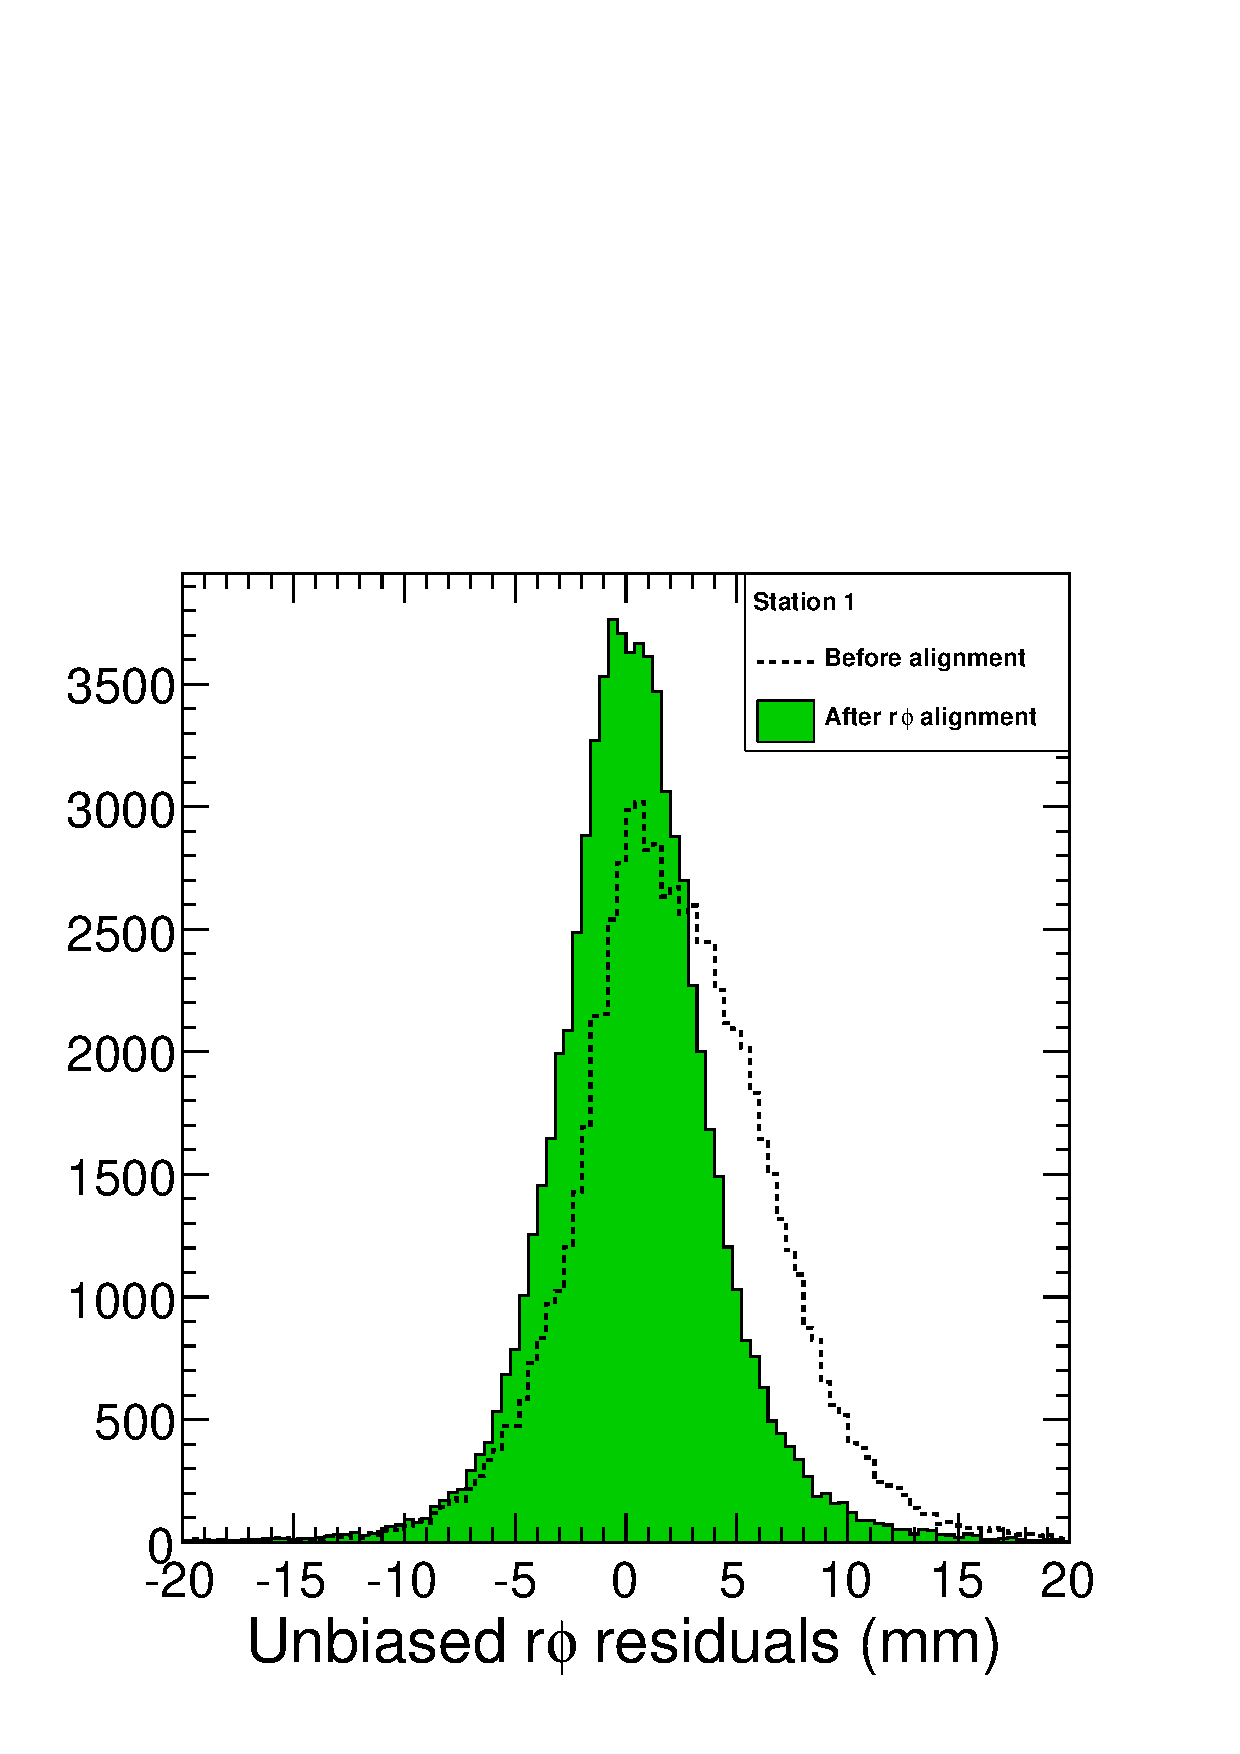
\includegraphics[width=\linewidth]{residuals_station1.pdf}

\vspace{0.5 cm}
Station 3

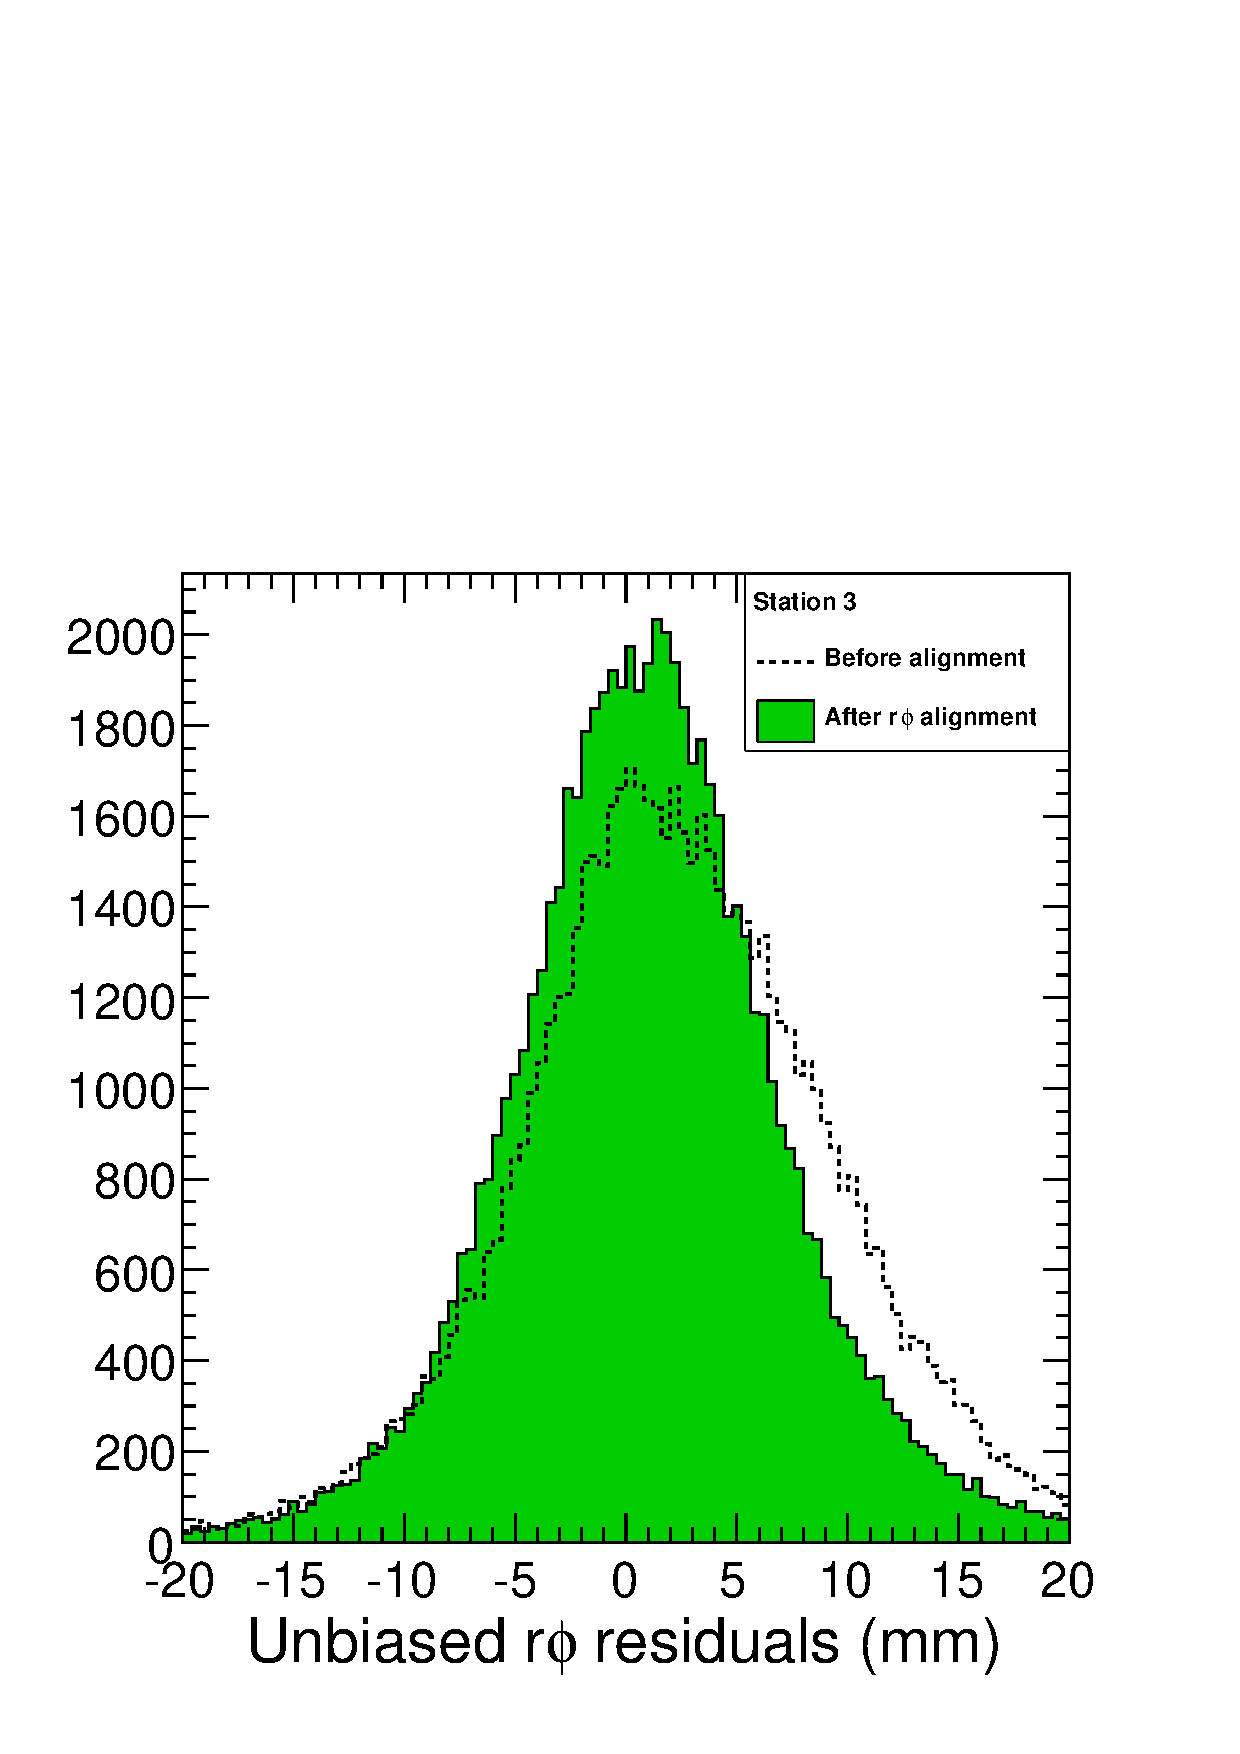
\includegraphics[width=\linewidth]{residuals_station3.pdf}

\column{0.3\linewidth}
Station 2
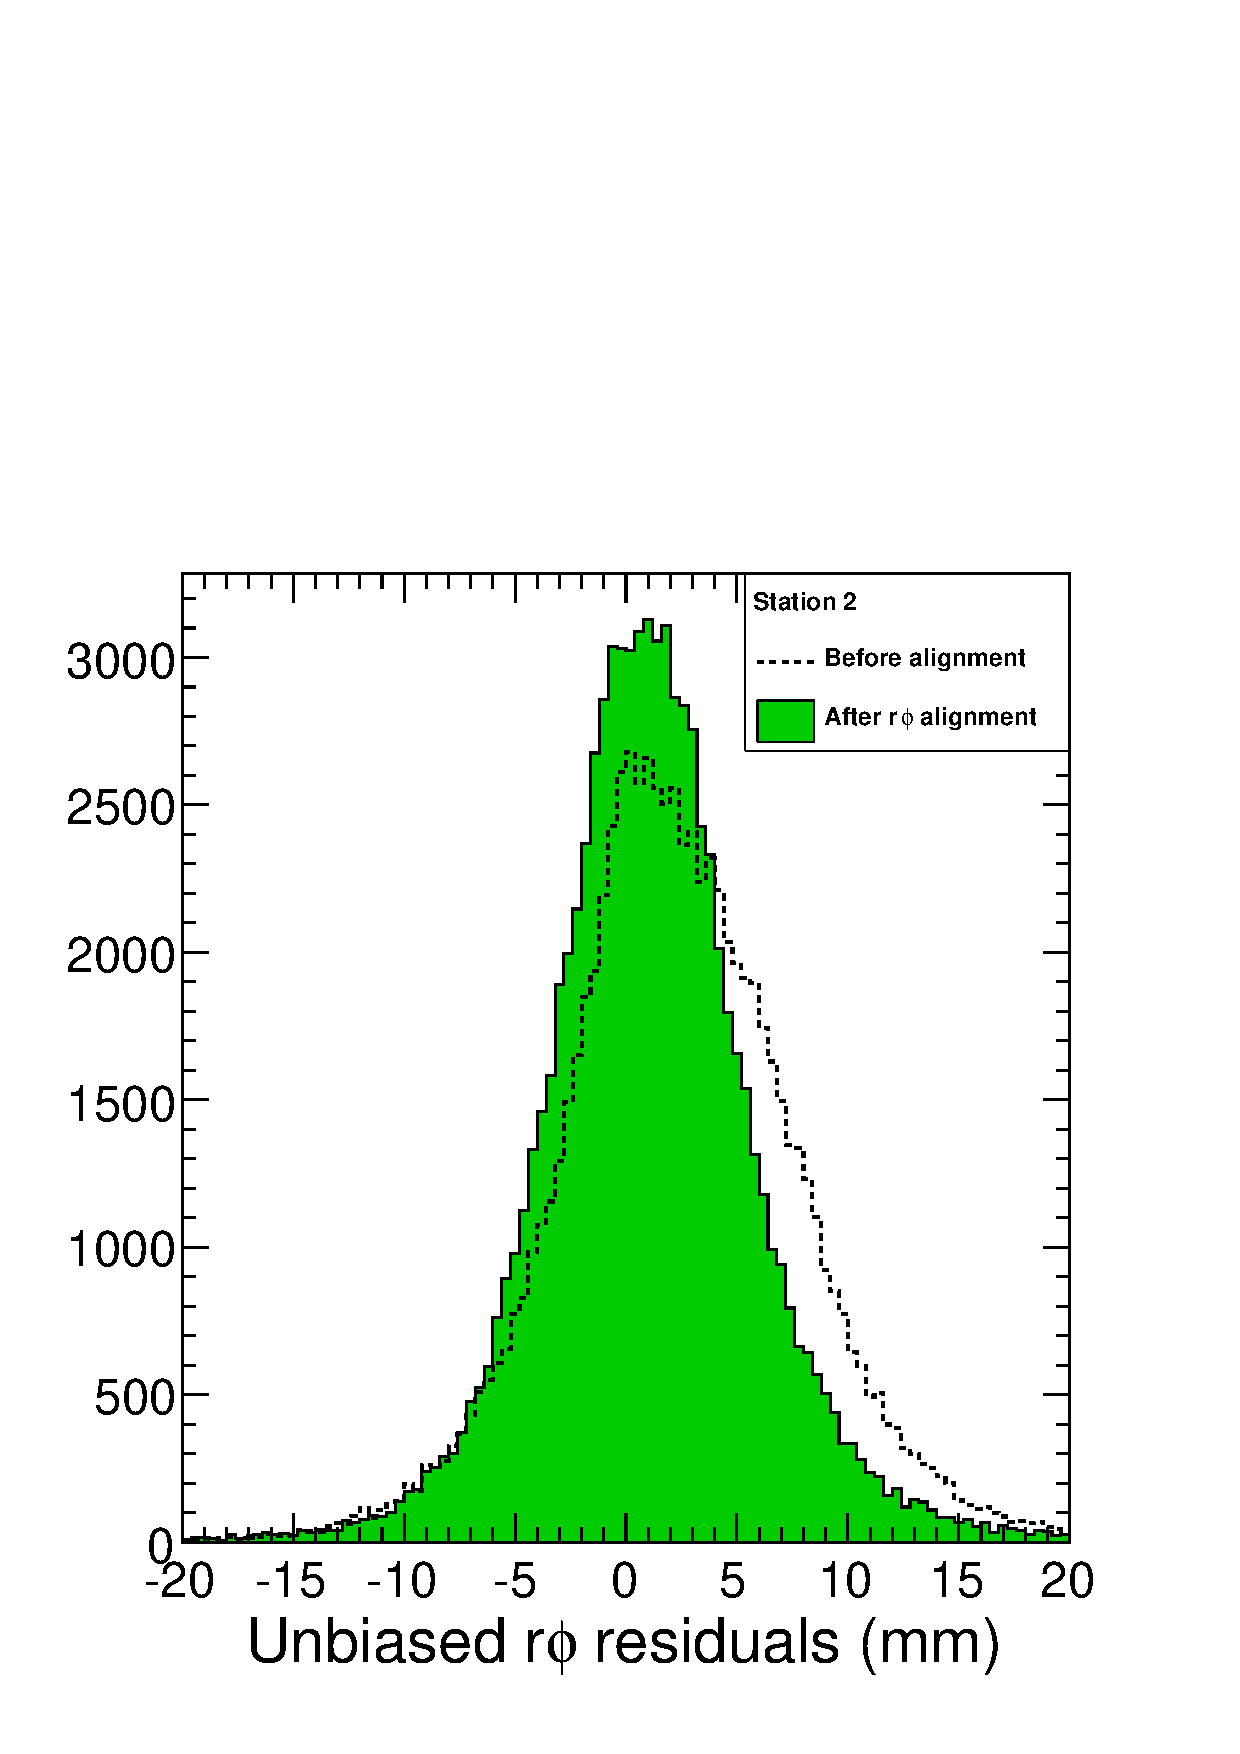
\includegraphics[width=\linewidth]{residuals_station2.pdf}

\vspace{0.5 cm}
Station 4
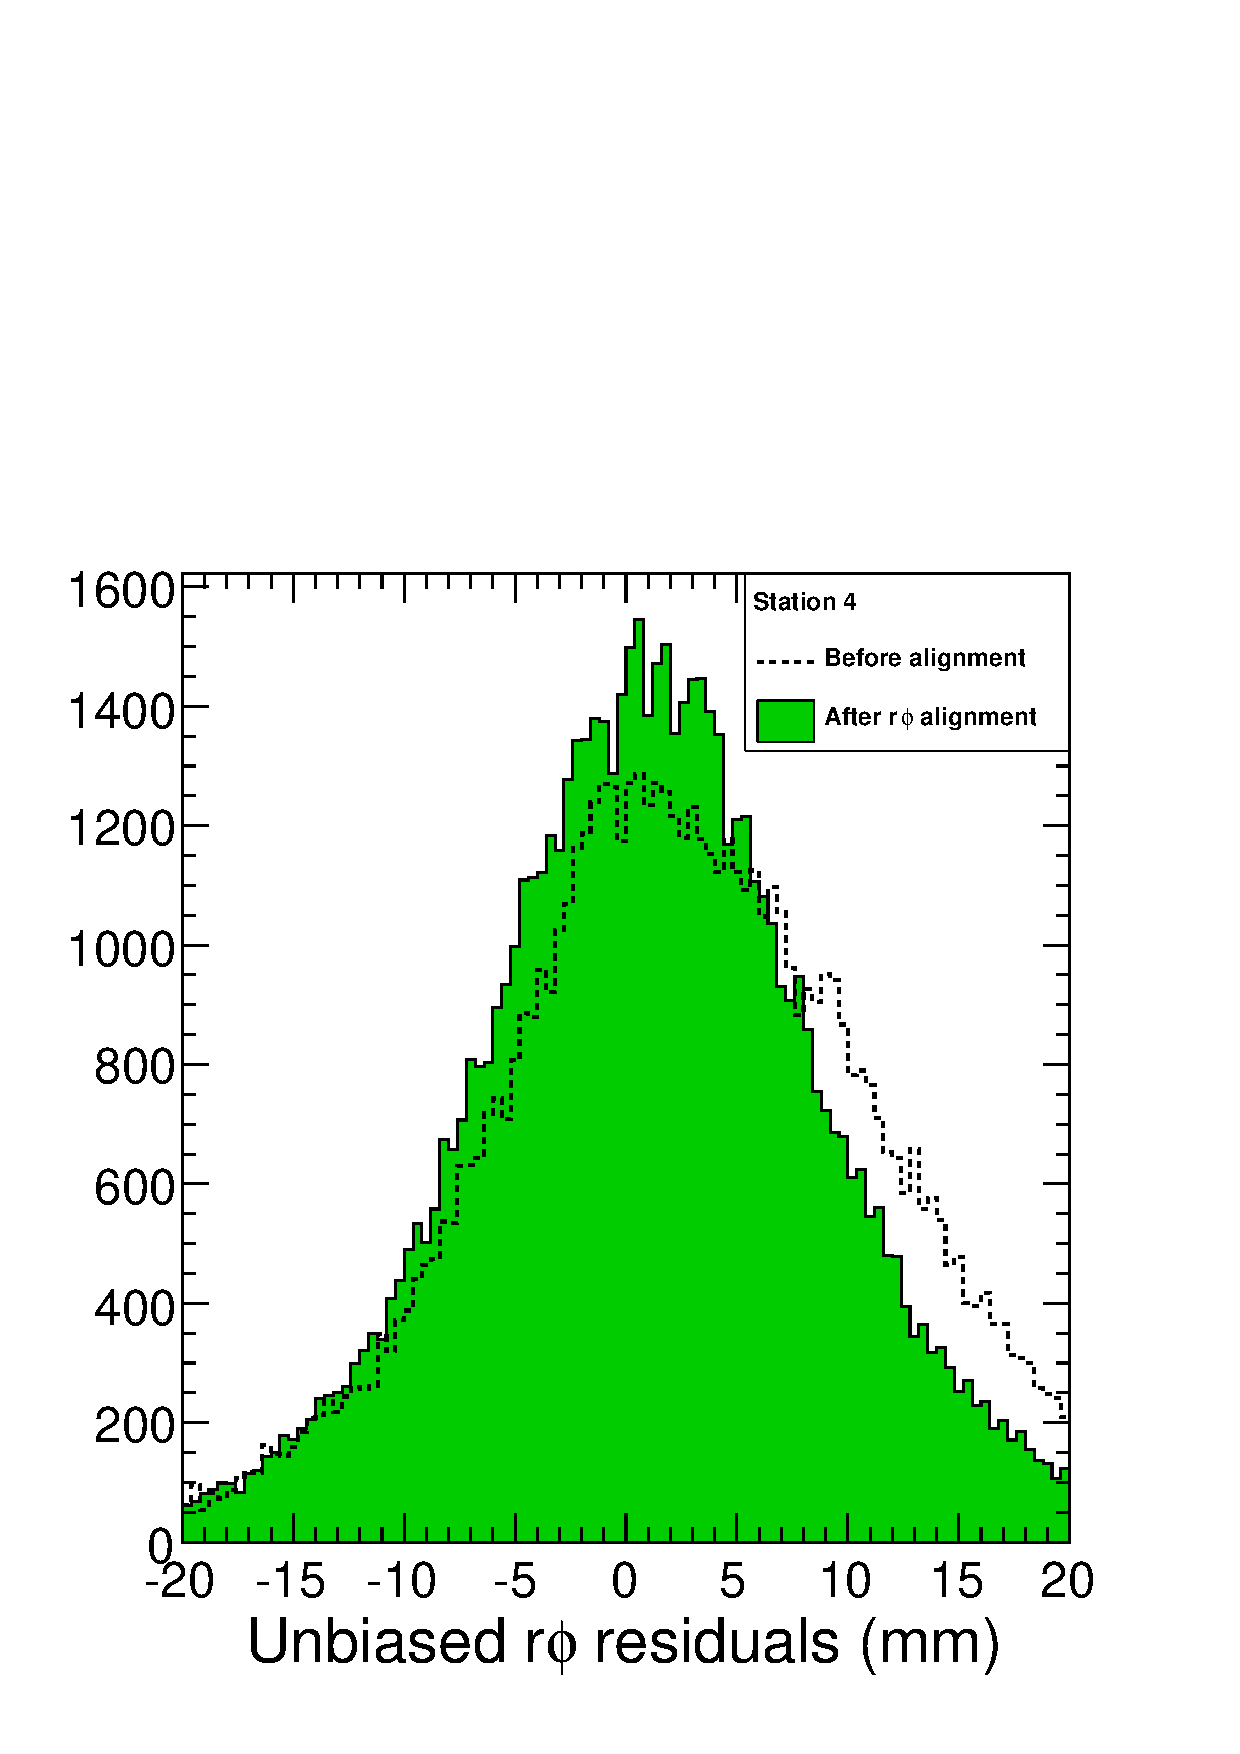
\includegraphics[width=\linewidth]{residuals_station4.pdf}

\column{0.3\linewidth}
\begin{itemize}
\item Not everyone can look at all the hundreds of plots
\item Summarize with raw residuals distributions
\item Not a very sensitive measure because chamber corrections are
  smaller than intrinsic width
\end{itemize}
\end{columns}

\end{frame}

\begin{frame}
\frametitle{Other evident effects}
\begin{itemize}
\item This was a local $x$ alignment only; there is no barrier to
  aligning $x$, $y$, and $\phi_z$ (the three most important
  parameters)
\begin{itemize}
\item I have such an alignment partially validated, but not in time for this meeting (and way too late for Javier)
\end{itemize}

\item Very important: the ``sawtooth mountain'' structure is due to a non-alignment effect.  The only misalignments that can cause it are
\begin{itemize}
\item radial, or local $z$: causes a linear slope in local $x$ residuals vs.\ local $x$ and local $y$ residuals vs.\ local $y$
\begin{itemize}
\item both cannot be accomodated with a local $z$ correction \mbox{(I tried it)\hspace{-1 cm}}
\end{itemize}
\item a $\phi_y$ misalignment of 70~mrad (unbelievable)
\item by process of elimination, it is not a misalignment
\end{itemize}

\item Note that the slope is {\it the same for all chambers}
\begin{itemize}
\item conclusion: it is a deformation of the chambers themselves, chambers are too narrow by 5~mm along the $x$ dimension \\
(or too wide--- I've made sign mistakes before)

\item it is the largest remaining effect in the width of the DT residuals distribution
\end{itemize}
\end{itemize}
\label{numpages}
\end{frame}

%% \section*{First section}
%% \begin{frame}
%% \begin{center}
%% \Huge \textcolor{blue}{First section}
%% \end{center}
%% \end{frame}

%% \begin{frame}
%% \frametitle{Conclusions}
%% \begin{itemize}
%% \item That's our suggestion
%% \end{itemize}
%% \end{frame}

\end{document}
